% !TeX root = mos-he.tex

%%%%%%%%%%%%%%%%%%%%%%%%%%%%%%%%%%%%%%%%%%%%%%%%%%%%%%%%%%%%%%%%

\begin{prob}{ימי הולדת זהים}{S}{(Birthday pairings)}

בחר באקראי 
$23$
אנשים ושאל כל אחד ליום ההולדת שלו. הנח התפלגות אחידה של 
$365$
ימי ההולדת השונים (אף אחד לא נולד ב-%
$29$
לפברואר). הראה שההסתברות שלפחות שניים מהם יהיו יום הולדת זהה היא גדולה מ-%
$0.5$.
\end{prob}

\solution{}

נחשב את ההסתברות ש-%
\textbf{אף אחד}
מה-%
$23$
אין ימי הולדת זהים ונראה שהיא פחות מ-%
$0.5$.
בחר יום הולדת ראשון בצורה אקראית, את יום ההולדת הבא בחר מתוך שאר הימים, את יום ההולדת הבא בחר מתוך שאר הימים, כך הלאה:
\[
\renewcommand*{\arraystretch}{2.5}
\begin{array}{rcl}
P(\textrm{אין זוג עם ימי הולדת זהים})&=&
  \overbrace{\disfrac{365}{365}\cdot\frac{364}{365}
  \cdot\frac{363}{365}\cdot \;\cdots \; \cdot \frac{344}{365}
  \cdot\frac{343}{365}}^{23\;\textrm{\small fractions}}\\
&=&\disfrac{365!}{365^{23}\cdot 342!}\approx 0.4927\,.
\end{array}
\]
רוב האנשים מנחשים שצריכים יותר מ-%
$23$
כדי למוצא שניים עם ימי הולדת זהים.

מחשבון מודרני מסוגל לחשב את ההסתברות, אבל שווה לחשבה באמצעות הקירוב של 
\L{Stirling}
שהוא
$\ln n! \approx n\ln n - n$:
\[
\renewcommand*{\arraystretch}{2}
\begin{array}{rcl}
\ln P(\textrm{אין זוג עם ימי הולדת זהים})&=&
  \ln\left(\disfrac{365!}{342!\cdot 365^{23}}\right)=\ln 365! - \ln 342! -23 \ln 365\\
&\approx& (365\ln 365 -365) - (342\ln 342 -342) - 23\,\ln 365 \\
&\approx&-0.7404\\
P(\textrm{אין זוג עם ימי הולדת זהים})&\approx&e^{-0.7404}=0.4769\,.
\end{array}
\]
הקורא מוזמן לחשב את ההסתברות עם הקירוב המדוייק יותר:
\[
\ln n!  \approx n\ln n - n + \frac{1}{6}\left(8n^3+4n^2+n+\frac{1}{30}\right)+\frac{1}{2}\ln\pi\,.
\]
\textbf{סימולציה}
\selectlanguage{english}
\begin{verbatim}
For 21 people:
Expectation of no pairs = 0.5563
Average no pairs        = 0.5497
For 22 people:
Expectation of no pairs = 0.5243
Average no pairs        = 0.5237
For 23 people:
Expectation of no pairs = 0.4927
Average no pairs        = 0.4933
For 24 people:
Expectation of no pairs = 0.4617
Average no pairs        = 0.4576
For 25 people:
Expectation of no pairs = 0.4313
Average no pairs        = 0.4345
\end{verbatim}
\selectlanguage{hebrew}

%%%%%%%%%%%%%%%%%%%%%%%%%%%%%%%%%%%%%%%%%%%%%%%%%%%%%%%%%%%%%

\begin{prob}{למצוא עמית ליום ההולדת}{S}{(Finding your birthmate)}

\textbf{עמית יום הולדת},
בקיצור עמית, הוא אדם עם ביום הולדת זהה לשלך.

מדוע מציאת עמית היא בעיה שונה ממציאת זוג עם ימי הולדת זהים?

\que{1}
כמה אנשים עליך לשאול כדי שההסתברות למציאת עמית גבוהה מ-%
$0.5$?

\que{2}
פתור את הבעיה על ידי שימוש במשוואה%
~\ref{eq.reciprocal} 
(עמוד%
~\L{\pageref{eq.reciprocal}}).
\end{prob}

\solution{}

להרבה אנשים יכול להיות יום הולדת זהה שנחשב כהצלחה במציאת זוג, אבל לא הצלחה במציאת עמית אלא אם יום ההולדת שלו זהה לשלך.

\ans{1}
מצא את המספר הקטן של אנשים כך ההסתברות שאף אחד מהם הוא עמית היא פחות מ-%
$0.5$.
ההסתברות שהאדם הראשון שאתה שואל אינו עמית היא
$364/365$,
אבל זאת גם ההסתברות שהשני, השלילי, 
\ldots, 
אינו עמית. הפתרון הוא ה-%
$k$
הקטן ביותר כך ש:
\[
P(\textrm{לא נמצא עמית})=\left(\frac{364}{365}\right)^k<\frac{1}{2}\,,
\]
which is $k=253$:
\[
\left(\frac{364}{365}\right)^{253} \approx 0.4995\,.
\]
\ans{2}
משוואה%
~\ref{eq.reciprocal}
היא:
\[
\lim_{n\rightarrow\infty}\left(\frac{n-1}{n}\right)^{n}=\frac{1}{e}\,,
\]
וניתן להשתמש בה לחשב את ההסתברות:
\begin{eqn}
P(\textrm{לא נמצא עמית})&=&
  \left(\disfrac{365-1}{365}\right)^k=\left[\left(\disfrac{364}{365}\right)^{365}\right]^{k/365}\\
&\approx& e^{-k/365}\\
e^{-253/365}&\approx&0.5000\,.
\end{eqn}
\textbf{סימולציה}
\selectlanguage{english}
\begin{verbatim}
For 251 people:
Probability of no match = 0.5023
Proportion no match     = 0.5120
For 252 people:
Probability of no match = 0.5009
Proportion no match     = 0.5055
For 253 people:
Probability of no match = 0.4995
Proportion no match     = 0.4984
For 254 people:
Probability of no match = 0.4982
Proportion no match     = 0.4987
For 255 people:
Probability of no match = 0.4968
Proportion no match     = 0.5078
\end{verbatim}
\selectlanguage{hebrew}

%%%%%%%%%%%%%%%%%%%%%%%%%%%%%%%%%%%%%%%%%%%%%%%%%%%%%%%%%%%%%

\begin{prob}{השוואת הבעיות יום הולדת זהה ועמית ליום ההולדת}{}{\\(Relating the birthday pairings and the birthmate problems)}

תהי 
$P_{\textrm{\footnotesize זוג}}(r)$
ההסתברות שמתוך 
$r$
אנשים לשניים יש יום הולדת זהה (בעיה~$31$), ותהי
$P_{\textrm{\footnotesize עמית}}(n)$
ההסתברות שמתוך
$n$
אנשים לפחות אחד הוא עימית שלך (בעיה~$32$).
נתון
$r$
עבור איזה
$n$,
$P_{\textrm{\footnotesize זוג}}(r) \approx P_{\textrm{\footnotesize עמית}}(n)$?
\end{prob}

\solution{1}

הפתרון מבוסס על
\L{\cite{birthday}}.

סמן ב-%
$P_{\textrm{\footnotesize זוג}}(r)$
את המשלים ל-%
$P_{\textrm{\footnotesize אין זוג}}(r)$.
מהפתרון לבעיית%
~$31$
מתקבל:
\[
\renewcommand*{\arraystretch}{2.2}
\begin{array}{lcl}
P_{\textrm{\footnotesize זוג אין}}(r)&=&
\disfrac{365}{365}\cdot 
  \frac{365-1}{365}\cdot \frac{365-2}{365} \cdot\;
  \cdots \;\cdot \frac{365-(r-1)}{365}\\
&=&1\left(1-\disfrac{1}{365}\right)
  \left(1-\disfrac{2}{365}\right) \cdot\;
  \cdots \;\cdot \left(1-\disfrac{r-1}{365}\right)\\
&\approx&1-\disfrac{1}{365} - \disfrac{2}{365} -
  \cdots - \disfrac{r-1}{365}\\
&=&1-\disfrac{1+2+3+\cdots + (r-1)}{365}\\
&=&1-\disfrac{r(r-1)/2}{365}\,,
\end{array}
\]
כאשר הקירוב במשוואה השלישית מתקבל מהשמטת חזקות של
$1/365$
גדולות מאחת כי הן קטנות מדי להשפיע באופן מהותי על התוצאה.

נסמן ב-%
$P_{\textrm{\footnotesize עמית אין}}(n)$
את המשלים ל-%
$P_{\textrm{\footnotesize עמית}}(n)$
ונשתמש באותו קירוב. מהפתרון לבעיה%
~$32$
נקבל:
\[
\renewcommand*{\arraystretch}{2.2}
\begin{array}{lcl}
P_{\textrm{\footnotesize עמית אין}}(n)
&=&\overbrace{\left(1-\frac{1}{365}\right)
  \left(1-\frac{1}{365}\right)\cdots
  \left(1-\frac{1}{365}\right)}^{n}\\
&\approx& 1-\overbrace{\frac{1}{365}-\frac{1}{365}\cdots-
  \frac{1}{365}}^{n}\\
&\approx& 1-\disfrac{n}{365}\\
\end{array}
\]
לכן
$P_{\textrm{\footnotesize זוג אין}}(r)\approx P_{\textrm{\footnotesize עמית אין}}(n)$
כאשר:
\[
n=\frac{r(r-1)}{2}\,.
\]
עבור
$r=23$, $n=(23\cdot 22)/2=253$.

\solution{2}

\L{Mosteller} \L{\cite[p.~322]{birthday}}
מביא את הפתרון האיטואיטיבי שלהלן:
\begin{quote}
כאשר משווים בין בעיית הזוג ובעיית העמית, אנו שמים לב שעבור 
$r$
אנשים בבעיית הזוג, קיימים 
$r(r-1)/2$
זוגות או 
\textbf{הזדמנויות}
לידי הולדת זהים; לעומת זאת, אם שואלים 
$n$
בבעיית העמית, קיימות רק 
$n$
הזדמנויות כדי שאמצא עמית אחד או יותר.
\end{quote}
מכאן הוא מסיק ש-%
$n\approx r(r-1)/2$.

ניתן להבין את הטיעון כך: בבעיית הזוג, בחר תאריך שרירותי ושאל אם לשניים מתוך
$r$
\textbf{תאריך זה}
הוא יום ההולדת שלהם. יש
\[
{r \choose 2}=\frac{r!}{2!(r-2)!} = \frac{r(r-1)}{2}
\]
דרכים שזה אפשרי. עבור בעיית העמית, יום ההולדת שלך נתון. יש אפשרות שלכל אחד מתוך
$n$
אנשים יש את אותו יום הולדת. על ידי השוואת שני ביוטיים נקבל 
$n$
עבורו
$P_{\textrm{\footnotesize זוג}}(r) \approx P_{\textrm{\footnotesize עמית}}(n)$.

תוכל להריץ את הסימולציות לבעיות
~$31, 32$
ולבדוק תוצאה זו.

%%%%%%%%%%%%%%%%%%%%%%%%%%%%%%%%%%%%%%%%%%%%%%%%%%%%%%%%%%%%%

\begin{prob}{חופש בימי הולדת}{D,S}{(Birthday holidays)}

בית חרושת נסגר בכל יום שהוא יום הולדת של אחד העובדים. אין חופשות נוספות.

\que{1} 
כמה עובדים כדי להעסיק כדי לקבל את מספר ימי-העבודה המקסימליים בשנה אחת?

\que{2}
מה התוחלת של היחס בין מספר ימי-העבודה המקסימליים לבין
$365^2$, 
מספר ימי-העבודה עם כל אחד מ-%
$365$
העובדים עובדים כל יום?

\textbf{רמז:}
הוכח שחייב להיות מקסימום על ידי בדיקת מקרי הקצה. אחר כך פתח נוסחה של התוחלת של ימי-העבודה ביום אחד.
\end{prob}

\solution{}

\ans{1}
בקצה אחד אם יש רק עובד אחד, יהיו 
$364$
ימי-עבודה. אם יש שני עובדים מספר ימי-העבודה הוא
$363+363=726$
(כאשר נתעלם המאפשרות הזניחה שלשניהם אותו יום הולדת). בקצה השני אם יש מיליון עובדים, מספר ימי-העבודה יהיה אפס כמעט בוודאות. אם מספר ימי-העבודה עולה ואחר כך חוזר לאפס, חייב להיות מקסימום בין הקצבות.

כדי לפשט את הסימונים, נסמן את המספר הימים בשנה ב-%
$N$
ומספר העובדים ב-%
$n$.

לכל יום נתון ההסתברות שהוא יום-עבודה היא ההסתברות שלכל עובד יום הולדת בתאריך אחר:
\[
P(\textrm{עבודה יום הוא נתון יום})=\overbrace{\disfrac{N-1}{N} \cdot \;\cdots\;\cdot \disfrac{N-1}{N}}^n = \left(1-\disfrac{1}{N}\right)^n\,.
\]
סמן ב-%
$p$ 
את
$\left(1-\disfrac{1}{N}\right)$.
אזי:
\[
E(\textrm{נתון ליום ימי-עבודה}) = n \cdot p^n + 0\cdot (1-p^n) = np^n\,.
\]
לכל ימי השנה אותה תוחלת כך שרק נותר להכפיל ב-%
$N$
כדי לקבל את התוחלת לשנה:
\begin{equation}\label{eq.holidays}
E(\textrm{לשנה ימי-עבודה}) = Nnp^n\,.
\end{equation}
כדי למצוא את המקסימום נגזור את משוואה%
~\ref{eq.holidays}
ביחס ל-%
$n$
ונשמתש ב-%
$(p^n)'=p^n\ln p$
ניתן להוכיח בעזרת כלל השרשרת:
\[
(p^n)' = ((e^{\ln p})^n)' =
(e^{n\ln p})' =
e^{n\ln p} (n\ln p)'=
(e^{\ln p})^n \ln p = p^n\ln p\,.
\]
הנגזרת של משוואה%
~\ref{eq.holidays}

היא:
\[
(Nnp^n)'= N (p^n + n (p^n)') = N (p^n + np^n\ln p)\,,
\]
שהיא $0$ כאשר:
\[
n=-\disfrac{1}{\ln p}\,.
\]
עבור
$N=365$
מתקבל
$n=364.5$
אבל
$n$
הוא מספר שלם ולכן המקסימום מתקבל ב-%
$n=364$
או
$n=365$
שנותנים אותו תוחלת של ימי-עבודה:
\begin{eqn}
E(\textrm{לשנה ימי-עבודה}) &=&Nnp^n\\
&=&365\cdot 364 \cdot \left(\disfrac{364}{365}\right)^{364}\\
&=&365\cdot 364  \cdot \disfrac{365}{365}\left(\disfrac{364}{365}\right)^{364}\\
&=&365\cdot 365  \cdot \left(\disfrac{364}{365}\right)^{365}\\
&=&48944\,.
\end{eqn}

\ans{2}
התוחלת של היחס היא:
\[
E(\textrm{מקסימליים ימי-עבודה}/\textrm{אפשריים ימי-עבודה})
=\disfrac{365\cdot 365  \cdot \left(\frac{364}{365}\right)^{365}}{365\cdot 365}=\left(\disfrac{364}{365}\right)^{365}\approx 0.3674\,.
\]
לפי משוואה%
~\ref{eq.reciprocal}:
\[
\lim_{n\rightarrow\infty}
E(\textrm{מקסימליים ימי-עבודה}/\textrm{אפשריים ימי-עבודה})
=\lim_{N\rightarrow \infty} \left(1-\disfrac{1}{N}\right)= \disfrac{1}{e}\,.
\]

\textbf{סימולציה}
\selectlanguage{english}
\begin{verbatim}
For 100 people
Expectation work-days    =  27742
Average work days        =  27743
Ratio work-days / 365**2 = 0.2082
For 250 people
Expectation work-days    =  45958
Average work days        =  45939
Ratio work-days / 365**2 = 0.3450
For 364 people
Expectation work-days    =  48944
Average work days        =  48936
Ratio work-days / 365**2 = 0.3674
For 365 people
Expectation work-days    =  48944
Average work days        =  48917
Ratio work-days / 365**2 = 0.3674
\end{verbatim}
\selectlanguage{hebrew}

%%%%%%%%%%%%%%%%%%%%%%%%%%%%%%%%%%%%%%%%%%%%%%%%%%%%%%%%%%%%%

\begin{prob}{על שפת התהום}{S}{(The cliff-hanger)}
חלקיק מוצב על ציר ה-%
$x$
במקום
$1$.
בכל מקום על ציר ה-%
$x$
הוא יכול לצעוד צעד ימינה עם הסתברות
$2/3$
וצעד שמאלה עם הסתברות
$1/3$
(איור%
~\ref{f.ruin1}).

\que{1}
מה ההסתברות שהחלקיק יגיע למקום
$0$
בסופו של דבר?

\que{2}
אם ההסתברות של צעד ימינה היא
$p$
וההסתברות של צעד שמאלה היא
$1-p$,
מה ההסתברות שהחלקיק יגיע למקום
$0$
בסופו של דבר? נתח את האפשרויות לערכים שונים של
$p$.

\textbf{רמז:}
השתשמש בהסתרויות מותנות לאחר הצעד הראשון.
\begin{figure}[tb]
\begin{center}
\begin{tikzpicture}[scale=1.5]
\draw (0,0) -- (6,0);
\draw[dashed] (6,0) -- (8,0) node[right] {$\infty$};
\foreach \x in {0,1,2,3,4,5,6} {
  \draw (\x,0) -- +(0,4pt);
  \node at (\x,-10pt) { $\x$ };
}
\draw[fill] (1,5mm) circle[radius=.5pt];
\draw[->] (1,5mm) -- node[above] {$1/3$} (0,5mm);
\draw[->,very thick] (1,5mm) -- node[above] {$2/3$} (2,5mm);

\foreach \x/\y in {2/10mm,3/15mm,4/20mm} {
  \draw[fill] (\x,\y) circle[radius=.5pt];
  \draw[->] (\x,\y) -- node[above] {$1/3$} (\x-1,\y);
  \draw[->] (\x,\y) -- node[above] {$2/3$} (\x+1,\y);
}
\end{tikzpicture}
\end{center}
\caption{?האם חלקיק יכול להגיע ל-$0$ (הציר אינסופי לימין)}\label{f.ruin1}
\end{figure}

\end{prob}

\solution{}

ניתן את הפרתונות של שתי השאלות ביחד כי חישוב ההסתברות ל-%
$p$
לא קשה יותר מחישוב ל-%
$p=2/3$.

\ans{1,2}
ננסה לחשב את ההסתברות בצורה ישירה. נסמן צעד שמאלה ב-%
$L$
וצעד ימינה ב-%
$R$.
החלקיק יכול להגיע ל-%
$0$
ישירות על ידי צעד
$L$
עם הסתברות
$\frac{1}{3}$,
או על ידי צעד
$RLL$
עם הסתברות
$\frac{2}{3}\cdot\frac{1}{3}\cdot\frac{1}{3}$,
או על ידי צעד
$RRLLL$
עם הסתברות
$\left(\frac{2}{3}\right)^2\left(\frac{1}{3}\right)^3$, \ldots\ .
החישוב נראה כמו סידרה הנדסית פשוטה אבל הוא מתעלם האפשרויות כגון
$RLRLL$.

נחשב את ההתסתברות שהחלקיק מגיעה ל-%
$0$
מ-%
$1$
בתלות בצעד הראשון:
\begin{eqn}
P(1\textrm{מ-}\;0 \textrm{ל- מגיע}) &=& 
P(1\textrm{מ-}\;0 \textrm{ל- מגיע}|\textrm{שמאלה ראשון צעד}) +\\
&&P(1\textrm{מ-}\;0 \textrm{ל- מגיע}|\textrm{ימינה ראשון צעד})\\
&=& (1-p)\cdot 1 + pP(2\textrm{מ-}\;1 \textrm{ל- מגיע})P(1\textrm{מ-}\;0 \textrm{ל- מגיע})\,.
\end{eqn}
אבל ההסתברות להגיע ל-%
$1$
מ-%
$2$
היא בדיוק ההסתברות להגיע ל-%
$0$
מ-%
$1$. 
נסמן ב-%
$P$
את 
$P(1\textrm{מ-}\;0 \textrm{ל- מגיע})$
ונקבל:
\begin{eqn}
P &=& (1-p) + pP^2\\
pP^2 - P + (1-p) &=&0\\
P&=& \frac{1\pm\sqrt{1-4p(1-p)}}{2p}\\
P&=&1,\; (1-p)/p\,.
\end{eqn}
אם
$p\leq 1/2$
אזי
$(1-p)/p\geq 1$, 
כך ש-%
$P=1$
הוא הפתרון היחיד ובטוח שהחלקיק יגיע ל-%
$0$.

אם 
$p=1$
אזי
$P=0$
כי אם החלקיק תמיד צועד ימינה הוא לא יכול להחזוור ל-%
$0$.

נניח ש-%
$P=1$
עבור
$1/2<p < 1$,
כלומר,
$P$
\textbf{לא תלוי ב-}$p$.
אבל 
$P$
לא יכול "לקפוץ" פתאום מ-%
$1$
ל-%
$0$
כאשר
$p$
שואף ל-%
$1$:
באיור%
~\ref{f.ruin2}
הקו האדום המקווקוו והנקודה האדומה ב-%
$(1,0)$.
לכן, עבור
$p> 1/2$
הפתרון היחיד הוא
$P=(1-p)/p< 1$.\footnote{\L{Mosteller}
כותב שזה נובע מרציפות אבל הוא לא מספק הוכחה.}

\begin{figure}[tb]
\begin{center}
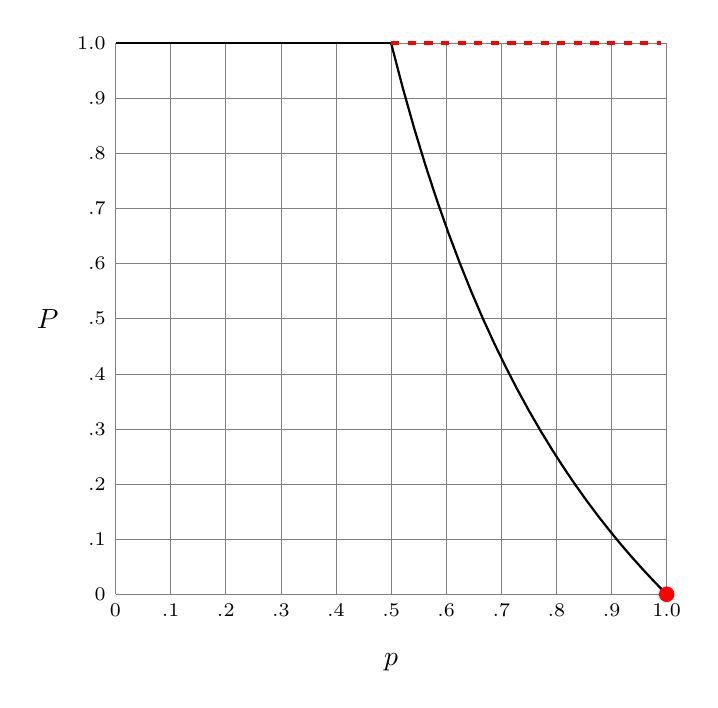
\begin{tikzpicture}[scale=7]
\draw[help lines,step=.1] (0,0) grid (1,1);
\foreach \x in {0,.1,.2,.3,.4,.5,.6,.7,.8,.9,1.0}
  \node[below] at (\x,0) {$\scriptstyle \x$};
\foreach \y in {0,.1,.2,.3,.4,.5,.6,.7,.8,.9,1.0}
  \node[left] at (0,\y) {$\scriptstyle \y$};
\draw[domain=0:.5,thick] plot (\x,1);
\draw[domain=.5:1,thick] plot (\x,{(1-\x)/\x});
\node at (.5,-3.5pt) {$p$};
\node at (-3.5pt,.5) {$P$};
\draw[ultra thick,red,dashed] (.5,1) -- +(.49,0);
\fill[red] (1,0) circle[radius=.4pt];
\end{tikzpicture}
\end{center}
\caption{הגרף של $P=\min(p/(1-p),1)$ עבור $p\in [0,1]$}\label{f.ruin2}
\end{figure}
עבור
$p=2/3, P=1/2$
ועבור
$p=1/2, P=1$.
זאת תוצאה מפתיעה כי לא היינו מצפים שהחלקיק יחזור תמיד ל-%
$0$
אם כיוון הצעד נקבע על ידי הטלת מטבע הוגן! אנו זקוקים למטבע ממש לא-הוגן (הסתברות של "עץ" שווה ל-%
$2/3$)
כדי להשוות את הסיכויים לחזור ל-%
$0$
או לא.

\textbf{סימולציה}
\selectlanguage{english}
\begin{verbatim}
For probability = 0.2500:
Probability of reaching 0 = 1.0000
Proportion reaching 0     = 1.0000
For probability = 0.5000:
Probability of reaching 0 = 1.0000
Proportion reaching 0     = 0.9612
For probability = 0.6667:
Probability of reaching 0 = 0.5000
Proportion reaching 0     = 0.5043
For probability = 0.7500:
Probability of reaching 0 = 0.3333
Proportion reaching 0     = 0.3316
For probability = 0.8000:
Probability of reaching 0 = 0.2500
Proportion reaching 0     = 0.2502
\end{verbatim}
\selectlanguage{hebrew}

%%%%%%%%%%%%%%%%%%%%%%%%%%%%%%%%%%%%%%%%%%%%%%%%%%%%%%%%%%%%%

\begin{prob}{המהמר פשט רגל}{D,S}{(Gambler's ruin)}
חלקיק מוצב על ציר ה-%
$x$
במקום
$m\geq 1$.
בכל מקום על ציר ה-%
$x$
הוא יכול לצעוד צעד ימינה עם הסתברות
$p>1/2$
וצעד שמאלה עם הסתברות
$1-p$.

\que{1}
מה ההסתברות שהחלקיק יגיע למקום
$0$
בסופו של דבר?

\que{2} יהי 
$n>m$.
אם החלקיק מגיע למקום 
$0$
או למקום
$n$
הוא מפסיק לצעוד (איור%
~\ref{f.ruin3}).
מה ההסתברות שהחלקיק יגיע למקום 
$0$?
מה ההסתברות שהחלקיק יגיע למקום
$n$
בסופו של דבר?
\begin{figure}[tb]
\begin{center}
\begin{tikzpicture}[scale=1.5]
\draw (0,0) -- (6,0);
\foreach \x in {0,1,2,3,4,5,6} {
  \draw (\x,0) -- +(0,4pt);
  \node at (\x,-10pt) { $\x$ };
}
\node at (2,-20pt) {$m$};
\node at (6,-20pt) {$n$};
\draw[fill] (2,5mm) circle[radius=.5pt];
\draw[->] (2,5mm) -- node[above] {$1/3$} (1,5mm);
\draw[->] (2,5mm) -- node[above] {$2/3$} (3,5mm);
\end{tikzpicture}
\end{center}
\caption{האם החלקיק יכול לחזור ל-%
$0$ (ציר סופי)?}
\label{f.ruin3}
\end{figure}

\textbf{הערה:} 
בעיה~35 מייצגת מהמר המשחק עם כמות סופית של כסף נגד קזינו עם כמות בלתי מוגבלת של כסף. הבעיה מבקשת את ההסתברות שהמהמר יפסיד את כל כספו. בעיה זו מייצגת מהמר אחד עם 
$m$
שמשחק נגד מהמר שני עם 
$n-m$.
הבעיה מבקשת את ההסתברויות ש%
\textbf{אחד}
מהם מפסיד את כל כספו לשני.
\end{prob}

\solution{}

הפתרון מבוסס על
\L{\cite[Chapter~2, Example~4m]{ross}}.

\ans{1}
הבפתרון לבעיה~35 ראינו שעבור
$p>1/2$
(כאן ההנחה נתונה), אם חלקיק נמצא במקום 
$1$
ההסתברות שלו להגיע ל-%
$0$
היא
$r=(1-p)/p$.
סימון: תהי 
$P(i,j)$
ההסתברות להגיע מ-%
$i$
מ-%
$j$.
בגלל שההסתברות של חלקיק להגיע ממקום אחד לשני לא תלוי במקום האבסולוטי:
\begin{equation}
P(0,m)=P(m-1,m)P(m-2,m-1)\cdots P(1,2)P(0,1)=r^m\,.
\end{equation}

\ans{2} 
תהי
$P_i=P(n,i)$
וחשב אותה תוך שימוש בהסתברות מותנית:
\begin{eqn}
P_i &=& pP_{i+1} + (1-p)P_{i-1}\\
pP_{i+1}&=&1\cdot P_i - (1-p)P_{i-1}\\
pP_{i+1}&=&(p+(1-p))P_i - (1-p)P_{i-1}\\
p(P_{i+1}-P_i)&=&(1-p)(P_i-P_{i-1})\\
P_{i+1}-P_i&=&r(P_i-P_{i-1})\,.
\end{eqn}
$P_0=0$ 
כי אם החלקיק נמצא ב-%
$0$
הוא מפסיק לצעוד. לכן:
\begin{eqn}
P_2 - P_1 &=& r(P_1 - P_0) = rP_1\\
P_3 - P_2 &=& r(P_2 - P_1) = r^2P_1\\
\cdots &=&\cdots\\
P_i - P_{i-1} &=& r(P_{i-1} - P_{i-2}) = r^{i-1}P_1\,.
\end{eqn}
רוב הגורמים בצד השמאלי מצטמצמים כאשר מחברים את המשוואות:
\begin{eqn}
P_i - P_1 &=& P_1\sum_{j=2}^{i}r^{j-1}\\
&=& P_1 + P_1\sum_{j=2}^{i}r^{j-1} - P_1 \\
P_i&=& P_1\sum_{j=0}^{i-1}r^j =P_1\left(\frac{1-r^i}{1-r}\right)\,.
\end{eqn}
אם חלקיק נמצא ב-%
$n$
הוא כבר נמצא ב-%
$n$
כך ש-%
$P_n=1$:
\begin{eqn}
1 &=& P_1\left(\frac{1-r^n}{1-r}\right)\\
P_1 &=& \left(\frac{1-r}{1-r^n}\right)\,,
\end{eqn}
ולכן (בהוכחה סימטרית שמחליפה 
$p$
ו-%
$1-p$):
{
\addtolength{\arraycolsep}{-3pt}
\begin{eqnarray}
\label{eq.ruin1}P(n,i) &=& \left(\frac{1-r^{i}}{1-r^n}\right)\\
\label{eq.ruin2}P(0,i) &=& \left(\frac{1-(1/r)^{n-i}}{1-(1/r)^{n}}\right)\,.
\end{eqnarray}
}
הקורא מוזמן להראות שהסכום של משוואות
~\ref{eq.ruin1},~\ref{eq.ruin2}
הוא $1$ כלומר שמובטח שאחד המהמרים ינצח והשני יפסיד.

עבור
$m=1, n=3, p=2/3$:
\begin{eqn}
P(0,1) &=& \left(\frac{1-\left(\frac{1}{2}\right)^{1}}{1-\left(\frac{1}{2}\right)^{3}}\right)=\frac{4}{7}\\
P(3,1) &=& \left(\frac{1-2^{2}}{1-2^{3}}\right)=\frac{3}{7}\,.
\end{eqn}

\textbf{סימולציה}
\selectlanguage{english}
\begin{verbatim}
For probability = 0.6667:
Probability of reaching (0,10) from 1 = (0.4995,0.5005)
Proportion reaching     (0,10) from 1 = (0.5056,0.4944)
Probability of reaching (0,10) from 4 = (0.0616,0.9384)
Proportion reaching     (0,10) from 4 = (0.0643,0.9357)
Probability of reaching (0,10) from 6 = (0.0147,0.9853)
Proportion reaching     (0,10) from 6 = (0.0123,0.9877)
\end{verbatim}

\begin{verbatim}
For probability = 0.7500:
Probability of reaching (0,10) from 1 = (0.3333,0.6667)
Proportion reaching     (0,10) from 1 = (0.3395,0.6605)
Probability of reaching (0,10) from 4 = (0.0123,0.9877)
Proportion reaching     (0,10) from 4 = (0.0115,0.9885)
Probability of reaching (0,10) from 6 = (0.0014,0.9986)
Proportion reaching     (0,10) from 6 = (0.0015,0.9985)
\end{verbatim}
\selectlanguage{hebrew}
ככל שלמהמר בצד שמאל יש יותר והסתברות גבוהה היותר לנצח בכל צעד, כך ההסתברות שלו לנצח גדלה.

%%%%%%%%%%%%%%%%%%%%%%%%%%%%%%%%%%%%%%%%%%%%%%%%%%%%%%%%%%%%%

\begin{prob}{משחק נועז או משחק זהיר}{S}{(Bold play vs. cautious play)}
ברולט ניתן להמר שהכדור יפול בכיס המסומן במספר זוגי. ההסתברות היא 
$18/38$
כי יש
$18$
מספרים זוגיים,
$18$
מספרים אי-זוגיים ו-%
$2$
מספרים ירוקים עליהם הקזינו מנצח.

איזו מהאסטרגיות שלהלן עדיפה?
\begin{enumerate}
\item 
משחק נועז: להמר $20$ בסיבוב אחד.
\item
משחק זהיר: להמר $1$ בכל סיבוב עד שאתה מנצח או מפסיד $20$.
\end{enumerate}
\textbf{רמז:} 
השתמש בתוצאות של בעיה~36.
\end{prob}

\solution{}

ההסתברות לנצח עם משחק נועז היא
$18/38\approx 0.4737$.

ההסתברות לנצח עם משחק זהיר היא (משוואה~\ref{eq.ruin1}):
\begin{eqnarray*}
r&=&\frac{20}{38}\Big /\frac{18}{38}=\frac{20}{18}\\
P(40,20) &=&
\frac{1-(20/18)^{20}}{1-(20/18)^{40}}\approx 0.1084\,.
\end{eqnarray*}
ברור שמשחק נועז עדיף על משחק זהיר.

\L{Mosteller}
כותב שהסבר איטואטיבי לתוצאה זו היא שהימור בסיבובים רבים חושף את המהמר לאפשרות שהקזינו מצנח בהסתברות 
$2/38$.

\textbf{סימולציה}
\selectlanguage{english}
\begin{verbatim}
Probability of bold wins     = 0.4737
Proportion bold wins         = 0.4677
Probability of cautious wins = 0.1084
Proportion cautious wins     = 0.1094
\end{verbatim}
\selectlanguage{hebrew}

%%%%%%%%%%%%%%%%%%%%%%%%%%%%%%%%%%%%%%%%%%%%%%%%%%%%%%%%%%%%%

\refstepcounter{problem}

%%%%%%%%%%%%%%%%%%%%%%%%%%%%%%%%%%%%%%%%%%%%%%%%%%%%%%%%%%%%%

\begin{prob}{הכימאי המגושם}{S}{(The clumsy chemist)}

נתון מספר רב של מקלות מזכוכית באורף 
$1$.
קצה אחד צבוע באדום ושני בכחול. כאשר זורקים אותם על הרצפה, הם נשברים לשלושה חלקים עם התפלגות אחידה של האורכים
(\ref{f.rod1}).
מה התוחלת של אורכו של החלק בקצה הכחול?

\textbf{רמז:}
במקום מקלות ישרים הנח שקבלת טבעות זכוכית ללא סימנים שגם הם נשברים לשלושה החלקים
(\ref{f.rod2}).

\begin{figure}[tb]

\centering
\selectlanguage{hebrew}
\subcaptionbox{%
חלוקת מקל לשלושה חלקים%
\label{f.rod1}}
[.45\textwidth]
{
\centering

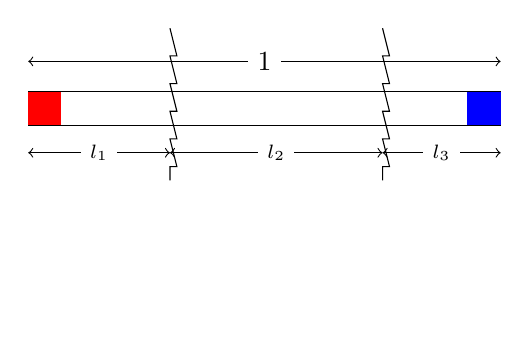
\begin{tikzpicture}
\draw (0,0) -- ++(6,0) -- ++(0,12pt) -- ++(-6,0) -- cycle;
\fill[red] (0,0) rectangle +(12pt,12pt);
\fill[blue] (6,0) rectangle +(-12pt,12pt);
\draw[<->] (0,23pt) --
  node[fill=white] {$1$} ++(6,0);
\draw[decorate,decoration=saw] (1.8,35pt) -- +(0,-55pt);
\draw[decorate,decoration=saw] (4.5,35pt) -- +(0,-55pt);
\draw[<->] (0,-10pt) --
  node[fill=white] {$\scriptstyle l_1$} (1.8,-10pt);
\draw[<->] (1.8,-10pt) --
  node[fill=white] {$\scriptstyle l_2$} (4.5,-10pt);
\draw[<->] (4.5,-10pt) --
  node[fill=white] {$\scriptstyle l_3$} (6,-10pt);
\path (0,-1) rectangle +(2,-1.5);
\end{tikzpicture}
}
\hspace{3em}
\subcaptionbox{%
חלוקת טבעת לשלושה חלקים%
\label{f.rod2}}
[.45\textwidth]
{
\centering
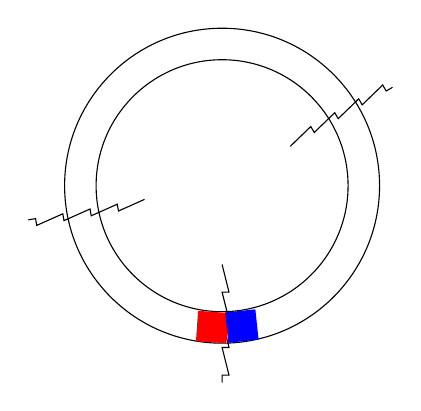
\begin{tikzpicture}
\draw (0,0) circle[radius=2];
\draw (0,0) circle[radius=1.6];
\draw[decorate,decoration=saw] (30:1) -- +(30:1.5);
\draw[decorate,decoration=saw] (190:1) -- +(190:1.5);
\draw[decorate,decoration=saw] (-90:1) -- +(-90:1.5);
\node[rotate=-4,fill=red,minimum width=11pt,minimum height=11pt]
  at (-94:1.8) {};
\node[rotate=6,fill=blue,minimum width=11pt,minimum height=11pt]
  at (-82:1.8) {};
\end{tikzpicture}
}
\end{figure}
\end{prob}

\solution{1}

אין סימטריה במלקות כי הקצות שונים מהחלק האמצני. אולם הטבעת סימטרית ולכן ההתפלגויות של שלושת החלקים יהיו אחידות עם תוחלת
$1/3$.
על ידי צביעת אחת מנקודות השבירה כפי שמופיע ב%
\ref{f.rod2},
הבעיה הופכת להיות זהה לבעיית המקל כך שההתפלגויות זהות. לכן התוחלת של אורכי החלקים היא גם
$1/3$.

\solution{2}

הפתרון אלגנטי שלהלן מבוסס על
\L{\cite{stack-rods}}.

נניח שהמקל מייצג את קטע הקו 
$(0,1)$.
המקל נשבר בשני מקומות שניתן לייצג בני משתנים אקראיים בלתי-תלויים עם התפלגות אחידה
$X,Y\in (0,1)$.
נחשב את ההסתברות
$P(|X-Y|>a)$.

טבלה%
~\ref{t.rods}
מראה נקודות 
$(x,y)$
כאשר
$x,y \in \{0.0, 0.1, 0.2, \ldots, 0.9\}$
והנקודה העשרונית הושמטה. הערכים בטבלה הם
$|X-Y|$.
עבור
$a=0.6$
הערכים למעלה משמאל מ-%
$(0,6)$--$(6,9)$,
והערכים למטה ומימין מ-%
$(6,0)$--$(9,6)$,
הם התוצאות שמגדירות את
$P(|X-Y|>a)$:
\[
P(|X-Y|>a)=2\cdot \frac{1}{2}(1-a)(1-a)=(1-a)^2\,.
\]
עבור
$a=0.6$, $P(|X-Y|>0.6)=(0.4)^2=0.16$.

\begin{table}[bt]
\[
\begin{array}{c}
\quad\\\\\\
a\\\\
\quad\\
y\\
\quad\\\quad\\\quad\\\quad
\end{array}
\begin{array}{|c|cccccccccc|}
\multicolumn{11}{l}{\qquad \qquad \qquad a}\\
\hline
9& 9 & 8 & 7 & 6 & 5 & 4 & 3 & 2 & 1 & 0  \\
8& 8 & 7 & 6 & 5 & 4 & 3 & 2 & 1 & 0 & 1  \\
7& 7 & 6 & 5 & 4 & 3 & 2 & 1 & 0 & 1 & 2  \\
6& 6 & 5 & 4 & 3 & 2 & 1 & 0 & 1 & 2 & 3  \\
5& 5 & 4 & 3 & 2 & 1 & 0 & 1 & 2 & 3 & 4  \\
4& 4 & 3 & 2 & 1 & 0 & 1 & 2 & 3 & 4 & 5  \\
3& 3 & 2 & 1 & 0 & 1 & 2 & 3 & 4 & 5 & 6  \\
2& 2 & 1 & 0 & 1 & 2 & 3 & 4 & 5 & 6 & 7  \\
1& 1 & 0 & 1 & 2 & 3 & 4 & 5 & 6 & 7 & 8  \\
0& 0 & 1 & 2 & 3 & 4 & 5 & 6 & 7 & 8 & 9  \\
\hline
&0 & 1 & 2 & 3 & 4 & 5 & 6 & 7 & 8 & 9  \\
\hline
\multicolumn{11}{c}{\quad \quad x\quad\quad\quad a}
\end{array}
\begin{array}{c}
\\\\\\
a\\\\
\end{array}
\]
\caption{התפלגות נקודות השבירה ב-%
$(0,1)\times (0,1)$}\label{t.rods}
\end{table}

המשלים הוא:
\[
P(|X-Y|<a)=1-(1-a)^2\,.
\]
הסתברות זו היא ההתפלגות ההסתברות המצטברת
\L{cumulative probability distribution (CPD)}
בקטע.
$(0,1)$.
ניתן לקבל את פונצקית הסתברות הצפיפות
\L{probability density function (PDF)}
על ידי גזירת ה-%
\L{CDP}:
\[
P(|X-Y|=a)= \frac{d}{da}P(|X-Y|<a) =
  \frac{d}{da}(1-(1-a)^2)=2(1-a)\,.
\]
התוחלת היא האינטגרל ה-%
\L{PDF}
כפול הערך:
\[
E(|X-Y|)= \int_{0}^{1} a\cdot2(1-a)\, da=
  2\left.\left(\frac{a^2}{2}-\frac{a^3}{3}\right)\right|_0^1=\frac{1}{3}\,.
\]

\textbf{סימולציה}
\selectlanguage{english}
\begin{verbatim}
Expectation of length of right piece = 0.3333
Average length of right piece        = 0.3359
\end{verbatim}
\selectlanguage{hebrew}

%%%%%%%%%%%%%%%%%%%%%%%%%%%%%%%%%%%%%%%%%%%%%%%%%%%%%%%%%%%%%

\begin{prob}{האס הראשון}{S}{(The first ace)}
חלק קלפים מחבילה מעורבת היטב עד שמופיע אס. מה התוחלת של מספר הקלפים שיש לחלק?

\textbf{רמז:}
חשוב על חבילה קלפים ללא האסים מסודרת בשורה.
\end{prob}

\solution{}
הקלפים הם כמו "מקל" באורך 
$48$
"שנשבר" על ידי 
$4$
ל-%
$5$
חלקים. הפתרון של בעיה~39 מתאים גם כאן והתוחלת של חלק היא
$48/5=9.6$.

\textbf{סימולציה}
\selectlanguage{english}
\begin{verbatim}
Expectation of first ace = 9.6000
Average first ace        = 9.5805
\end{verbatim}
\selectlanguage{hebrew}

%%%%%%%%%%%%%%%%%%%%%%%%%%%%%%%%%%%%%%%%%%%%%%%%%%%%%%%%%%%%%

